\documentclass[12pt,letterpaper]{hmcpset}
\usepackage[margin=1in]{geometry}
\usepackage{graphicx}
\usepackage{amsmath}
\usepackage{boxedminipage}
\usepackage{url}

% info for header block in upper right hand corner
\name{ }
\class{Math 45 - Section --- \hspace{20pt}}
\assignment{HW 04}
\duedate{Due: Tuesday, 2016-03-29}

\newcommand{\pn}[1]{\left( #1 \right)}
\newcommand{\abs}[1]{\left| #1 \right|}
\newcommand{\bk}[1]{\left[ #1 \right]}

\newcommand{\vb}{\mathbf{v}}
\newcommand{\ub}{\mathbf{u}}
\renewcommand{\labelenumi}{{(\alph{enumi})}}

\begin{document}

\problemlist{1, 2, 3, 4, 5, 6}

% 1 %
\begin{problem}[1]
A certain drug is being administered intravenously
  to a hospital patient who has had no prior drug treatments.  Fluid containing 5 mg/cm$^3$ of the drug
  enters the patient's bloodstream at a rate of 100 cm$^3$/hr. The
  drug is absorbed by tissues or otherwise leaves the bloodstream at a
  rate proportional to the amount present, with a rate constant of 0.4
  $(\mbox{hr})^{-1}$.
\begin{enumerate}
\item Assuming that the drug is always uniformly distributed
  throughout the bloodstream, write a differential equation for the
  amount of the drug that is present in the bloodstream at any time and state the initial condition.
\item Use the integrating factor method to solve this IVP.
\item How much of the drug is present in the bloodstream after a long
  time?
\end{enumerate}
\end{problem}

\begin{solution}
  \vfill
\end{solution}
\newpage

% 2 %
\begin{problem}[2]
Work this problem by hand (using calculators for arithmetic is fine).  Consider the IVP
$$y' =1-t+y, \qquad y(0)=1.$$	
\begin{enumerate}
	\item Use Euler's method with step-size $h=0.2$ to estimate the value of $y(1)$. Then, repeat for $h=0.1$. 
	\item Find the solution to the DE analytically (by hand) and use it to determine the exact value of $y(1)$.
	\item Show that halving the step-size $h$ roughly halves the error in your numerical approximations of $y(1)$.
\end{enumerate}
\end{problem}

\begin{solution}
  \vfill
\end{solution}
\newpage

% 3 %
\begin{problem}[3]
Consider the DE $y' = \cos(t)-y$.
\begin{enumerate}
  	\item Find the general solution to this ODE (by hand).
  	\item Generate the direction field and some solution curves
          for this DE with a range of different
          initial conditions using ODEToolkit (\url{http://odetoolkit.hmc.edu}), dfield
          (\url{http://math.rice.edu/~dfield/dfpp.html}), or
           equivalent piece of ODE software. Attach a printout with
          your homework.
  	\item Based on your numerical exploration in part (b), conjecture what happens to $y(t)$ as $t$ tends to infinity. Can you explain this behavior from the general solution you found in part (a)?
\end{enumerate}
\end{problem}

\begin{solution}
  \vfill
\end{solution}
\newpage

\begin{problem}[4]
Work this problem by hand (no computers allowed).
\begin{enumerate}
\item Sketch the direction field for the differential equation
$$y' = -\cfrac{x}{y}$$
for $x\in\left[-3,3\right]$ and $y\in\left[-3,3\right]$.  Make sure to indicate the direction field at all lattice points with integer coordinates. (You can skip $y=0$ since the DE is not defined there.)
\item If you were given the sketch of the direction field from part (a), but were not given the equation, how would you know that the DE was non-autonomous?
\end{enumerate}
\end{problem}

\begin{solution}
  \vfill
\end{solution}
\newpage

\begin{problem}[5]
You have been hired by a fishery to do some preliminary work on
  modeling a fish population under various harvesting strategies.
  They have asked you to start with this mathematical model that
  accounts for logistic growth, death, and harvesting:
\[
\frac {dP}{dt} = r P (1-P/K) - \alpha P - H(t,P).
\]
Here, $P(t)$ represents the fishery biomass (total mass of fish).  The
constant $r$ relates to the growth rate of your population, and $K$ is
the carrying capacity of your fishery---the maximum biomass that the
fishery can sustain. The term $-\alpha P$ accounts for the natural
death of your fish.  Assume $r$, $K$, $\alpha$, and $P(t)$ are all
positive.

The function $H(t,P)$ describes the harvesting of the fish. The fishery
wants to understand what would happen to the population of fish under
different scenarios.

\begin{enumerate}

\item The fishery hasn't actually started raising fish yet.  However,
  to perform your calculations and impress the fishery with your
  mathematical skills, it will be helpful to pick an organism to
  model.  So, pick your favorite aquatic organism to model, then come
  up with reasonable values for all of your parameters.  What units
  will they have? You can try to look up values on the Internet, or
  just make some reasonable estimates.

\item What initial condition(s) will you use?

\item First, consider harvesting strategies that are time invariant.
  In other words, consider only case where $H$ is not a function of
  time. Here are two natural choices for $H=H(P)$ in this case: the
  fishery could harvest at a constant rate (say $H=10 \text{kg per
    day}$) or it could harvest at a rate that is proportional to the
  fishery biomass (say 1\% of the biomass is harvested every month).
  In each of these two cases, calculate the long-term population of
  the fish, and the long-term harvesting rate.  Perform these
  calculations by hand.

\item In the case where $H=H_0$ is a constant, solve for $P(t)$
  analytically (by hand).  In addition, numerically approximate $P(t)$
  using Euler's Method (or any other numerical method of your choice)
  and verify that your analytic answer agrees with your numerical
  one.\\
\textbf{Note:} There is are some hints on how to analytically solve for $P(t)$ on our Sakai site. 

\item (Optional) Think of some other harvesting strategy that might be
  reasonable besides the two considered here.  Your $H(t,P)$ could
  involve time.  (Perhaps it changes with the season?)  Extend your
  numerical method so that it can also numerically approximate $P(t)$
  for your chosen harvesting function.

\end{enumerate}
\end{problem}
\newpage
\begin{solution}
	\vfill
\end{solution}
\newpage

\begin{problem}[6]
Examine Student Y's work on the following problem.  What did the student do correctly?  What mistake(s) did the student make?  What is a more correct response to the problem?  Come up with as many different explanations to help Student Y as you can. At the least, one explanation should involve the fact that the DE is autonomous and another should involve slope fields.

\begin{center}
\framebox{\parbox[c]{5.5in}{A population of fish satisfies the differential equation
\[
\frac{dP}{dt}=rP(1-P/K)-H_0
\]
where $P(t)$ represents the biomass of the fish (in pounds), $r$ represents a birth rate (in $1/\text{months}$), $K$ represents a carrying capacity of the environment, and $H_0$ represents a harvesting rate (in pounds/month). Sketch a reasonable guess for what $P(t)$ will look like for some $P(0)=P_0<K$.\\

\centering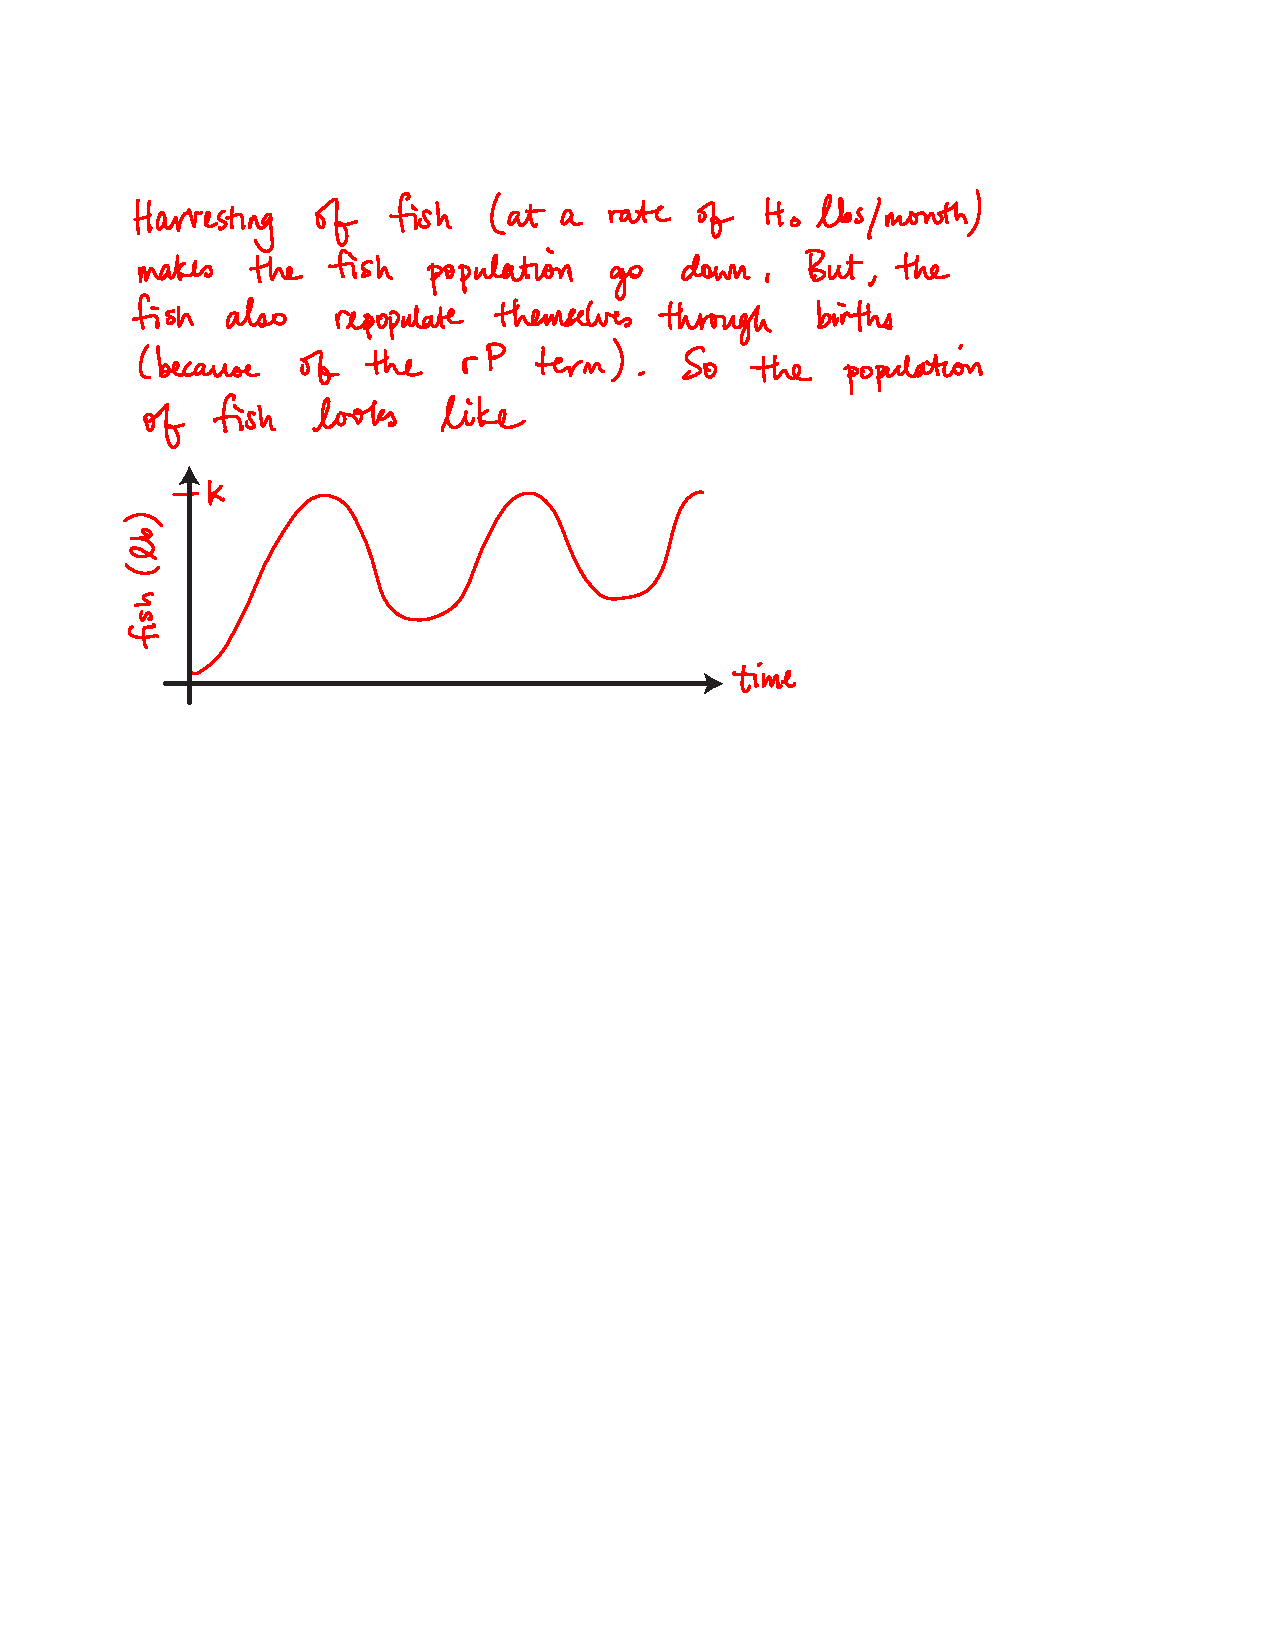
\includegraphics[width=4.5in,keepaspectratio=true]{45-hw04-misconception3}}}
\end{center}
\end{problem}

\begin{solution}
  \vfill
\end{solution}
\end{document}